\documentclass[
  oneside,
  degree=bachelor,
  fullwidthstop=false,
  fontset=none,
  times=false,
  minted=false,
  biblatex=false,
]{tongjithesis}

\usepackage{xeCJK}
\setCJKmainfont[
  Path=/System/Library/Fonts/Supplemental/,
  Extension=.ttc,
  FontIndex=3,
  BoldFont=Songti.ttc,
  BoldFeatures={FontIndex=1},
  AutoFakeBold=false
]{Songti.ttc}
\setCJKsansfont[
  Path=/System/Library/Fonts/,
  Extension=.ttc,
  FontIndex=1,
  BoldFont=STHeiti Medium.ttc,
  BoldFeatures={FontIndex=1}
]{STHeiti Light.ttc}
\setCJKmonofont{仿宋_GB2312}[Path=/Users/kinakoxu/Library/Fonts/,Extension=.ttf]
\setCJKfamilyfont{zhsong}[
  Path=/System/Library/Fonts/Supplemental/,
  Extension=.ttc,
  FontIndex=3,
  BoldFont=Songti.ttc,
  BoldFeatures={FontIndex=1},
  AutoFakeBold=false
]{Songti.ttc}
\setCJKfamilyfont{zhhei}[
  Path=/System/Library/Fonts/,
  Extension=.ttc,
  FontIndex=1,
  BoldFont=STHeiti Medium.ttc,
  BoldFeatures={FontIndex=1}
]{STHeiti Light.ttc}
\setCJKfamilyfont{zhkai}{楷体_GB2312}[Path=/Users/kinakoxu/Library/Fonts/,Extension=.ttf]
\setCJKfamilyfont{zhfs}{仿宋_GB2312}[Path=/Users/kinakoxu/Library/Fonts/,Extension=.ttf]
\providecommand{\songti}{\CJKfamily{zhsong}}
\providecommand{\heiti}{\CJKfamily{zhhei}}
\providecommand{\kaishu}{\CJKfamily{zhkai}}
\providecommand{\fangsong}{\CJKfamily{zhfs}}

\begin{document}

% ============================================================
%  封面信息
% ============================================================
\school{国豪书院}
\major{}
\student{2452627}{徐佳涛}
\thesistitle{机器人避障\\寻径问题}{}
\thesistitleeng{Design and Implementation of Robot Obstacle Avoidance Path Planning Algorithms}{A Comparative Study Based on Graph Search, Reinforcement Learning and Heuristic Methods}
\thesisadvisor{张红云}
\thesisdate{\the\year}{\the\month}{\the\day} % 使用当前日期; 也可以自定义日期

% ============================================================
%  信息说明页
% ============================================================

% 成果类型：design（毕业设计）或 thesis（毕业论文）
\infotype{thesis}

% 内容简述（请用300字以内简要概述）
\infoabstract{%
本文完成了机器人避障寻径课程设计。报告基于栅格地图实现了 BFS、A*、改进 A*、Q-Learning、人工势场法以及 Dijkstra 等算法，并设计了一个 30x30 的复杂场景用于测试。实验结果表明，BFS 与 Dijkstra 能稳定得到最短路，但搜索范围较大；A* 搜索效率更高；改进 A* 的综合路径代价更低；Q-Learning 经过训练后能够学得可行策略；人工势场法在复杂场景中容易陷入局部极小值。此外，程序还实现了 BFS、A* 和改进 A* 的搜索过程动态展示。
}

% 毕业设计：图纸数量与正文字数（成果类型为 design 时填写，两者须同时填写）
% \infodrawings{5}
% \infowordcount{15000}

% 毕业论文：正文总字数（成果类型为 thesis 时填写）
\infothesiswords{4500}

% 随附资料（每条用 \item 开头；不填则显示空白行）
\infomaterials{}

\MakeCover
\cleardoublepage

\tableofcontents
\cleardoublepage

\mainmatter
\chapter{问题背景与动态场景建模}\label{chap:background}

\section{问题背景}

机器人避障寻径问题的目标是在存在障碍物的环境中，为机器人规划一条从起点到终点的无碰撞路径。这个问题既是经典的图搜索问题，也和机器人导航、自动驾驶、仓储搬运等应用场景紧密相关。

本课程设计要求先完成 BFS 和 A* 两种基础算法，再在此基础上设计更复杂的场景，并尝试加入其他方法进行改进。为了让不同算法具有可比性，本文统一采用栅格地图作为环境模型，并在相同起点、终点和障碍分布下进行测试。

\section{栅格地图建模}

本文采用二维栅格地图表示机器人运动空间。地图中的每个网格单元只有两种状态：
\begin{enumerate}
  \item 空闲单元，记为 0，机器人可以通过；
  \item 障碍单元，记为 1，机器人不能进入。
\end{enumerate}

机器人状态定义为坐标 $(r,c)$，动作集合为
\begin{equation}
  \mathcal{A}=\{(-1,0),(1,0),(0,-1),(0,1)\},
\end{equation}
分别表示上、下、左、右四个方向移动。若下一状态越界或撞到障碍，则该动作无效。

\section{动态场景设计}

为了满足题目中“自主设计更高难度场景图”的要求，本文在原始 9$\times$8 基础场景外，又设计了一个 30$\times$30 的复杂场景。该场景的设计思路如下：

\begin{itemize}
  \item 通过多条横向、纵向长墙增加整体搜索深度；
  \item 利用少量门洞制造狭窄通道；
  \item 设计 U 型障碍和假通路，增加局部陷阱；
  \item 将起点和终点放置在对角区域，迫使算法进行全局搜索。
\end{itemize}

这里的“动态场景建模”主要体现在两点：一是地图规模从简单场景扩展到复杂场景；二是在搜索过程展示中，地图状态会随着访问节点和最终路径逐帧变化，从而形成动态演示效果。

\section{场景建模实现}

复杂场景的核心构造方式是先创建空白栅格，再按坐标填充障碍物和门洞。对应代码如下：

\begin{lstlisting}[language=Python,caption={30x30 场景图的构造方式},label={code:map}]
def get_challenge_map(size=30):
    grid = np.zeros((size, size), dtype=int)
    grid[0, :] = 1
    grid[-1, :] = 1
    grid[:, 0] = 1
    grid[:, -1] = 1

    for col, rows in vertical_walls.items():
        for row in rows:
            grid[row, col] = 1

    for row, cols in horizontal_walls.items():
        for col in cols:
            grid[row, col] = 1
\end{lstlisting}

通过这种方式，可以比较灵活地设计障碍布局，也方便后续测试不同算法在同一场景下的表现。

\chapter{项目结构与程序设计}\label{chap:structure}

\section{项目文件结构}

本次课程设计的主要程序文件如下：

\begin{itemize}
  \item \texttt{pathfinder.py}：主程序，负责 BFS、A*、改进 A*、Q-Learning、人工势场法的统一实验，以及结果图和 GIF 动画生成；
  \item \texttt{Dijikstra.py}：单独实现 Dijkstra 算法，并与 BFS、A* 进行对比；
  \item \texttt{robot\_search.py}：早期的基础地图验证脚本；
  \item 实验结果图：如 \texttt{challenge\_30x30\_comparison.png}、\texttt{challenge\_30x30\_q\_learning\_curve.png} 等。
\end{itemize}

\section{主程序设计思路}

为了便于对比多种算法，本文将主程序组织成统一框架。整体流程如下：

\begin{enumerate}
  \item 生成基础场景或 30x30 复杂场景；
  \item 调用不同算法进行寻路；
  \item 记录访问顺序、最终路径和综合代价；
  \item 输出对比表格、静态结果图和动态图。
\end{enumerate}

这种组织方式的优点是结构清晰，各算法共享同一套地图和评价指标，便于直接比较结果。

\section{核心模块划分}

从程序实现角度来看，整个系统主要分为以下几个模块：

\begin{itemize}
  \item \textbf{地图模块}：负责基础地图与复杂地图的构造；
  \item \textbf{搜索模块}：包括 BFS、A*、改进 A*、Dijkstra 等图搜索方法；
  \item \textbf{学习模块}：实现 Q-Learning 的训练和策略提取；
  \item \textbf{可视化模块}：负责静态图片与 GIF 动态展示的生成；
  \item \textbf{结果统计模块}：输出路径步数、访问节点数和综合代价。
\end{itemize}

\section{程序执行流程}

主程序的执行流程可以概括为“建图、搜索、统计、绘图”四个步骤。入口函数的组织如下：

\begin{lstlisting}[language=Python,caption={主程序的整体流程},label={code:main}]
def main():
    basic_grid, basic_start, basic_end = get_basic_map()
    basic_results = compare_on_map(basic_grid, basic_start, basic_end)

    challenge_grid, challenge_start, challenge_end = get_challenge_map()
    challenge_results = compare_on_map(
        challenge_grid, challenge_start, challenge_end
    )
\end{lstlisting}

从这个流程可以看出，程序对基础场景和复杂场景采用统一的测试逻辑，因此后续如果需要继续增加新场景或新算法，也比较方便扩展。

\chapter{算法设计}\label{chap:algorithm}

\section{BFS 算法}

广度优先搜索（BFS）按照层次逐层扩展节点。在单位代价栅格地图中，BFS 能保证第一次到达终点时得到最短路径。其优点是实现简单、结果稳定；缺点是搜索具有较强盲目性，在大场景中会访问大量无关节点。

\section{A* 算法}

A* 在一致代价搜索基础上加入启发式函数，评价函数定义为
\begin{equation}
  f(n)=g(n)+h(n),
\end{equation}
其中 $g(n)$ 表示起点到当前节点的实际代价，$h(n)$ 表示当前节点到终点的估计代价。本文选用曼哈顿距离作为启发式函数：
\begin{equation}
  h(n)=|r-r_g|+|c-c_g|.
\end{equation}

相较于 BFS，A* 的搜索方向更集中，因此通常访问节点更少。

\section{改进 A* 算法}

基础 A* 只关注路径长度，不考虑路径是否贴近障碍，也不考虑转弯是否过多。为此，本文在单步代价中加入贴障惩罚和转向惩罚：
\begin{equation}
  c(n_i,n_{i+1})=1+\lambda_1 p_{\text{obs}}+\lambda_2 p_{\text{turn}}.
\end{equation}

这种设计的目标不是一味追求最短长度，而是在路径长度、平滑性和安全性之间取得更平衡的结果。

\section{Q-Learning 算法}

Q-Learning 属于强化学习方法。它通过不断与环境交互，更新状态-动作价值函数：
\begin{equation}
  Q(s,a)\leftarrow Q(s,a)+\alpha \left[r+\gamma \max_{a'}Q(s',a')-Q(s,a)\right].
\end{equation}

本文中，状态为机器人当前位置，动作是四个移动方向。奖励函数同时考虑了到达终点奖励、撞墙惩罚、靠近终点奖励和重复访问惩罚，以提高训练效率。

\section{人工势场法}

人工势场法将终点看作吸引源，将障碍物看作排斥源，机器人在合成势场作用下向目标移动。它的优点是实现直观、局部反应速度快，但缺点也很明显，即在复杂障碍环境中容易陷入局部极小值。

\section{Dijkstra 算法}

Dijkstra 是求解非负权图最短路径的经典方法。在本文的单位代价栅格环境中，它可以看作不带启发式信息的一致代价搜索。它能够稳定得到最短路径，但在复杂场景中搜索效率通常低于 A*。

\section{算法比较}

不同算法的特点如\cref{tab:method-comparison} 所示。

\begin{table}[!htb]
  \centering
  \caption{各算法特点对比}\label{tab:method-comparison}
  \begin{tabular}{@{}p{2.3cm}p{2.6cm}p{3.3cm}p{4.6cm}@{}}
    \toprule
    \textbf{算法} & \textbf{是否保证最短路} & \textbf{主要优点} & \textbf{主要缺点} \\
    \midrule
    BFS & 是 & 实现简单，结果稳定 & 搜索盲目性强，复杂场景扩展节点多 \\
    Dijkstra & 是 & 适用于非负权图，理论清晰 & 不利用目标方向信息，效率偏低 \\
    A* & 是 & 搜索效率较高，适合静态已知地图 & 仅以距离为目标时，路径可能贴近障碍 \\
    改进 A* & 综合代价更优 & 路径更平滑、更安全 & 参数需要调节，未必扩展最少节点 \\
    Q-Learning & 训练充分时可获得可行策略 & 可学习策略，适合扩展到智能体方法 & 训练时间较长 \\
    人工势场法 & 否 & 实现简单，局部反应快 & 易陷入局部极小值 \\
    \bottomrule
  \end{tabular}
\end{table}

\chapter{核心代码实现}\label{chap:code}

\section{BFS 核心代码}

BFS 的核心思想是使用队列按层遍历。代码如下：

\begin{lstlisting}[language=Python,caption={BFS 的核心实现},label={code:bfs}]
def bfs_search(grid, start, end):
    queue = deque([start])
    visited = {start}
    came_from = {}

    while queue:
        current = queue.popleft()
        if current == end:
            return reconstruct_path(came_from, current)

        for nxt in get_neighbors(grid, current):
            if nxt not in visited:
                visited.add(nxt)
                came_from[nxt] = current
                queue.append(nxt)
\end{lstlisting}

\section{A* 核心代码}

A* 通过优先队列维护待访问节点，并用 $f=g+h$ 来确定扩展优先级。

\begin{lstlisting}[language=Python,caption={A* 的节点扩展逻辑},label={code:astar}]
def a_star_search(grid, start, end):
    open_set = []
    heapq.heappush(open_set, (0, start))
    g_score = {start: 0}

    while open_set:
        _, current = heapq.heappop(open_set)
        if current == end:
            return True

        for nxt in get_neighbors(grid, current):
            tentative_g = g_score[current] + 1
            heuristic = abs(nxt[0] - end[0]) + abs(nxt[1] - end[1])
            f_score = tentative_g + heuristic
            heapq.heappush(open_set, (f_score, nxt))
\end{lstlisting}

\section{改进 A* 核心代码}

改进 A* 主要体现在代价函数设计上，代码如下：

\begin{lstlisting}[language=Python,caption={改进 A* 的附加代价},label={code:improved-astar}]
step_cost = 1.0
step_cost += nearby_obstacle_penalty(grid, nxt)
if prev_dir is not None and direction != prev_dir:
    step_cost += 0.1

heuristic = manhattan(nxt, end)
heuristic += 0.2 * nearby_obstacle_penalty(grid, nxt)
f_score = tentative_g + heuristic_weight * heuristic
\end{lstlisting}

\section{Q-Learning 核心代码}

Q-Learning 通过奖惩更新 Q 表，代码如下：

\begin{lstlisting}[language=Python,caption={Q-Learning 的价值更新},label={code:qlearning}]
reward = self.step_reward(state, nxt, valid, seen)
best_next = np.max(self.q_table[nxt[0], nxt[1]])
td_target = reward + self.gamma * best_next
td_error = td_target - self.q_table[state[0], state[1], action]
self.q_table[state[0], state[1], action] += self.alpha * td_error
\end{lstlisting}

\section{Dijkstra 核心代码}

Dijkstra 的重点是按当前最小路径代价不断扩展节点：

\begin{lstlisting}[language=Python,caption={Dijkstra 的核心实现},label={code:dijkstra}]
priority_queue = [(0.0, start)]
distances = {start: 0.0}

while priority_queue:
    current_cost, current = heapq.heappop(priority_queue)
    if current == end:
        return True
    for neighbor in get_neighbors(grid, current):
        new_cost = current_cost + 1.0
        if new_cost < distances.get(neighbor, float("inf")):
            distances[neighbor] = new_cost
            heapq.heappush(priority_queue, (new_cost, neighbor))
\end{lstlisting}

\section{动态可视化核心代码}

动态展示的关键是根据访问顺序和路径回溯过程逐帧更新图像：

\begin{lstlisting}[language=Python,basicstyle=\footnotesize\ttfamily,caption={动态展示中的帧更新逻辑},label={code:gif}]
def update(frame_idx):
    display = np.copy(base_grid)

    for node in visited_frames[:frame_idx]:
        if node not in (start, end) and display[node] == 0:
            display[node] = 2

    if frame_idx >= len(visited_frames) and result.success:
        path_idx = frame_idx - len(visited_frames)
        for node in path_frames[:path_idx]:
            if node not in (start, end):
                display[node] = 3

    image.set_data(display)
    return [image]
\end{lstlisting}

\chapter{实验结果与动态可视化}\label{chap:experiment}

\section{实验环境}

本文实验在本地 Python 环境下完成，主要依赖 NumPy 与 Matplotlib 进行地图建模和可视化。实验环境配置如\cref{tab:env} 所示。

\begin{table}[!htb]
  \centering
  \caption{实验环境配置}\label{tab:env}
  \begin{tabular}{@{}ll@{}}
    \toprule
    \textbf{项目} & \textbf{配置} \\
    \midrule
    编程语言 & Python 3.13.9 \\
    数值计算库 & NumPy 2.3.5 \\
    可视化库 & Matplotlib 3.10.6 \\
    地图规模 & 9x8 与 30x30 \\
    动态展示方式 & 导出 GIF 动画文件 \\
    \bottomrule
  \end{tabular}
\end{table}

\section{基础场景结果}

在原始 9$\times$8 地图中，各算法结果如\cref{tab:basic-result} 所示。

\begin{table}[!htb]
  \centering
  \caption{基础场景实验结果}\label{tab:basic-result}
  \begin{tabular}{@{}lcccc@{}}
    \toprule
    \textbf{算法} & \textbf{是否成功} & \textbf{访问节点数} & \textbf{路径步数} & \textbf{综合代价} \\
    \midrule
    BFS & 是 & 57 & 20 & 20.00 \\
    A* & 是 & 32 & 20 & 27.20 \\
    改进 A* & 是 & 35 & 20 & 26.20 \\
    Q-Learning & 是 & 21 & 20 & 27.20 \\
    人工势场法 & 否 & 25 & 24 & -- \\
    \bottomrule
  \end{tabular}
\end{table}

\begin{figure}[!htb]
  \centering
  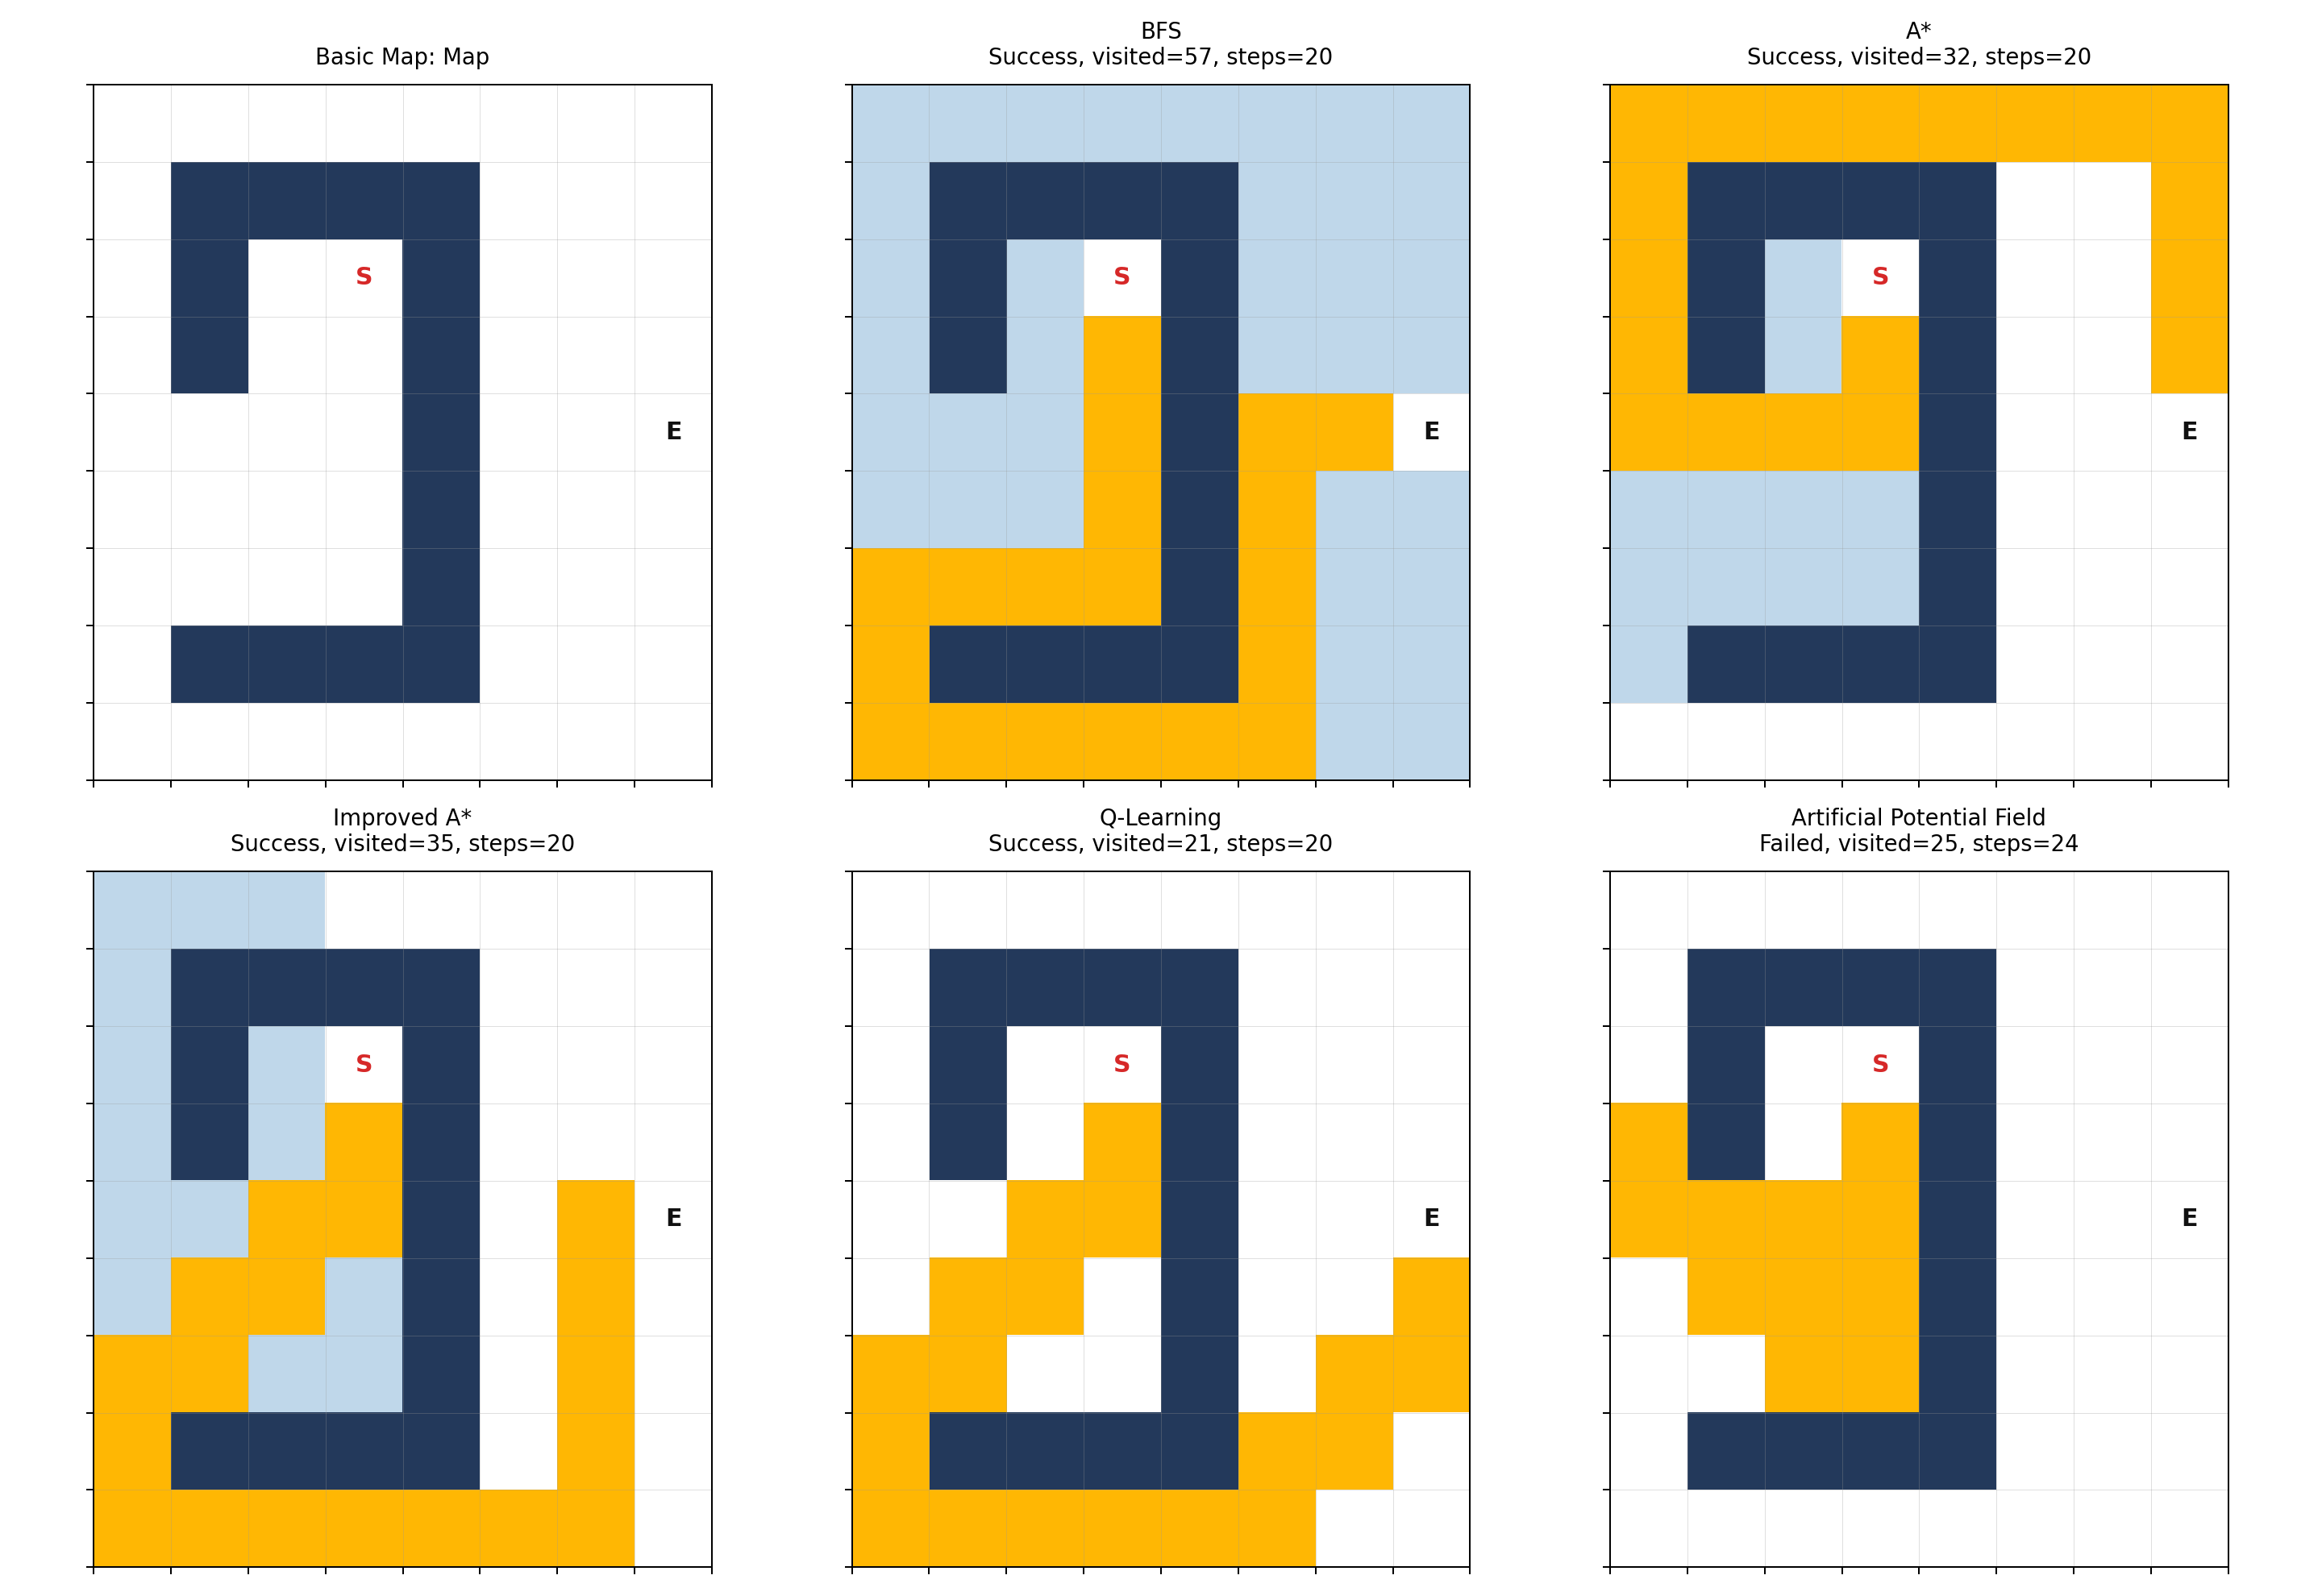
\includegraphics[width=0.85\textwidth]{../basic_map_comparison.png}
  \caption{基础场景下各算法结果对比}
  \label{fig:basic-comparison}
\end{figure}

\section{复杂场景结果}

在自主设计的 30$\times$30 复杂场景中，不同算法表现出更明显差异，如\cref{tab:challenge-result} 所示。

\begin{table}[!htb]
  \centering
  \caption{30x30 复杂场景实验结果}\label{tab:challenge-result}
  \begin{tabular}{@{}lcccc@{}}
    \toprule
    \textbf{算法} & \textbf{是否成功} & \textbf{访问节点数} & \textbf{路径步数} & \textbf{综合代价} \\
    \midrule
    BFS & 是 & 334 & 64 & 64.00 \\
    Dijkstra & 是 & 334 & 64 & 82.20 \\
    A* & 是 & 231 & 64 & 81.96 \\
    改进 A* & 是 & 263 & 64 & 79.56 \\
    Q-Learning & 是 & 65 & 64 & 81.64 \\
    人工势场法 & 否 & 91 & 90 & -- \\
    \bottomrule
  \end{tabular}
\end{table}

\begin{figure}[!htb]
  \centering
  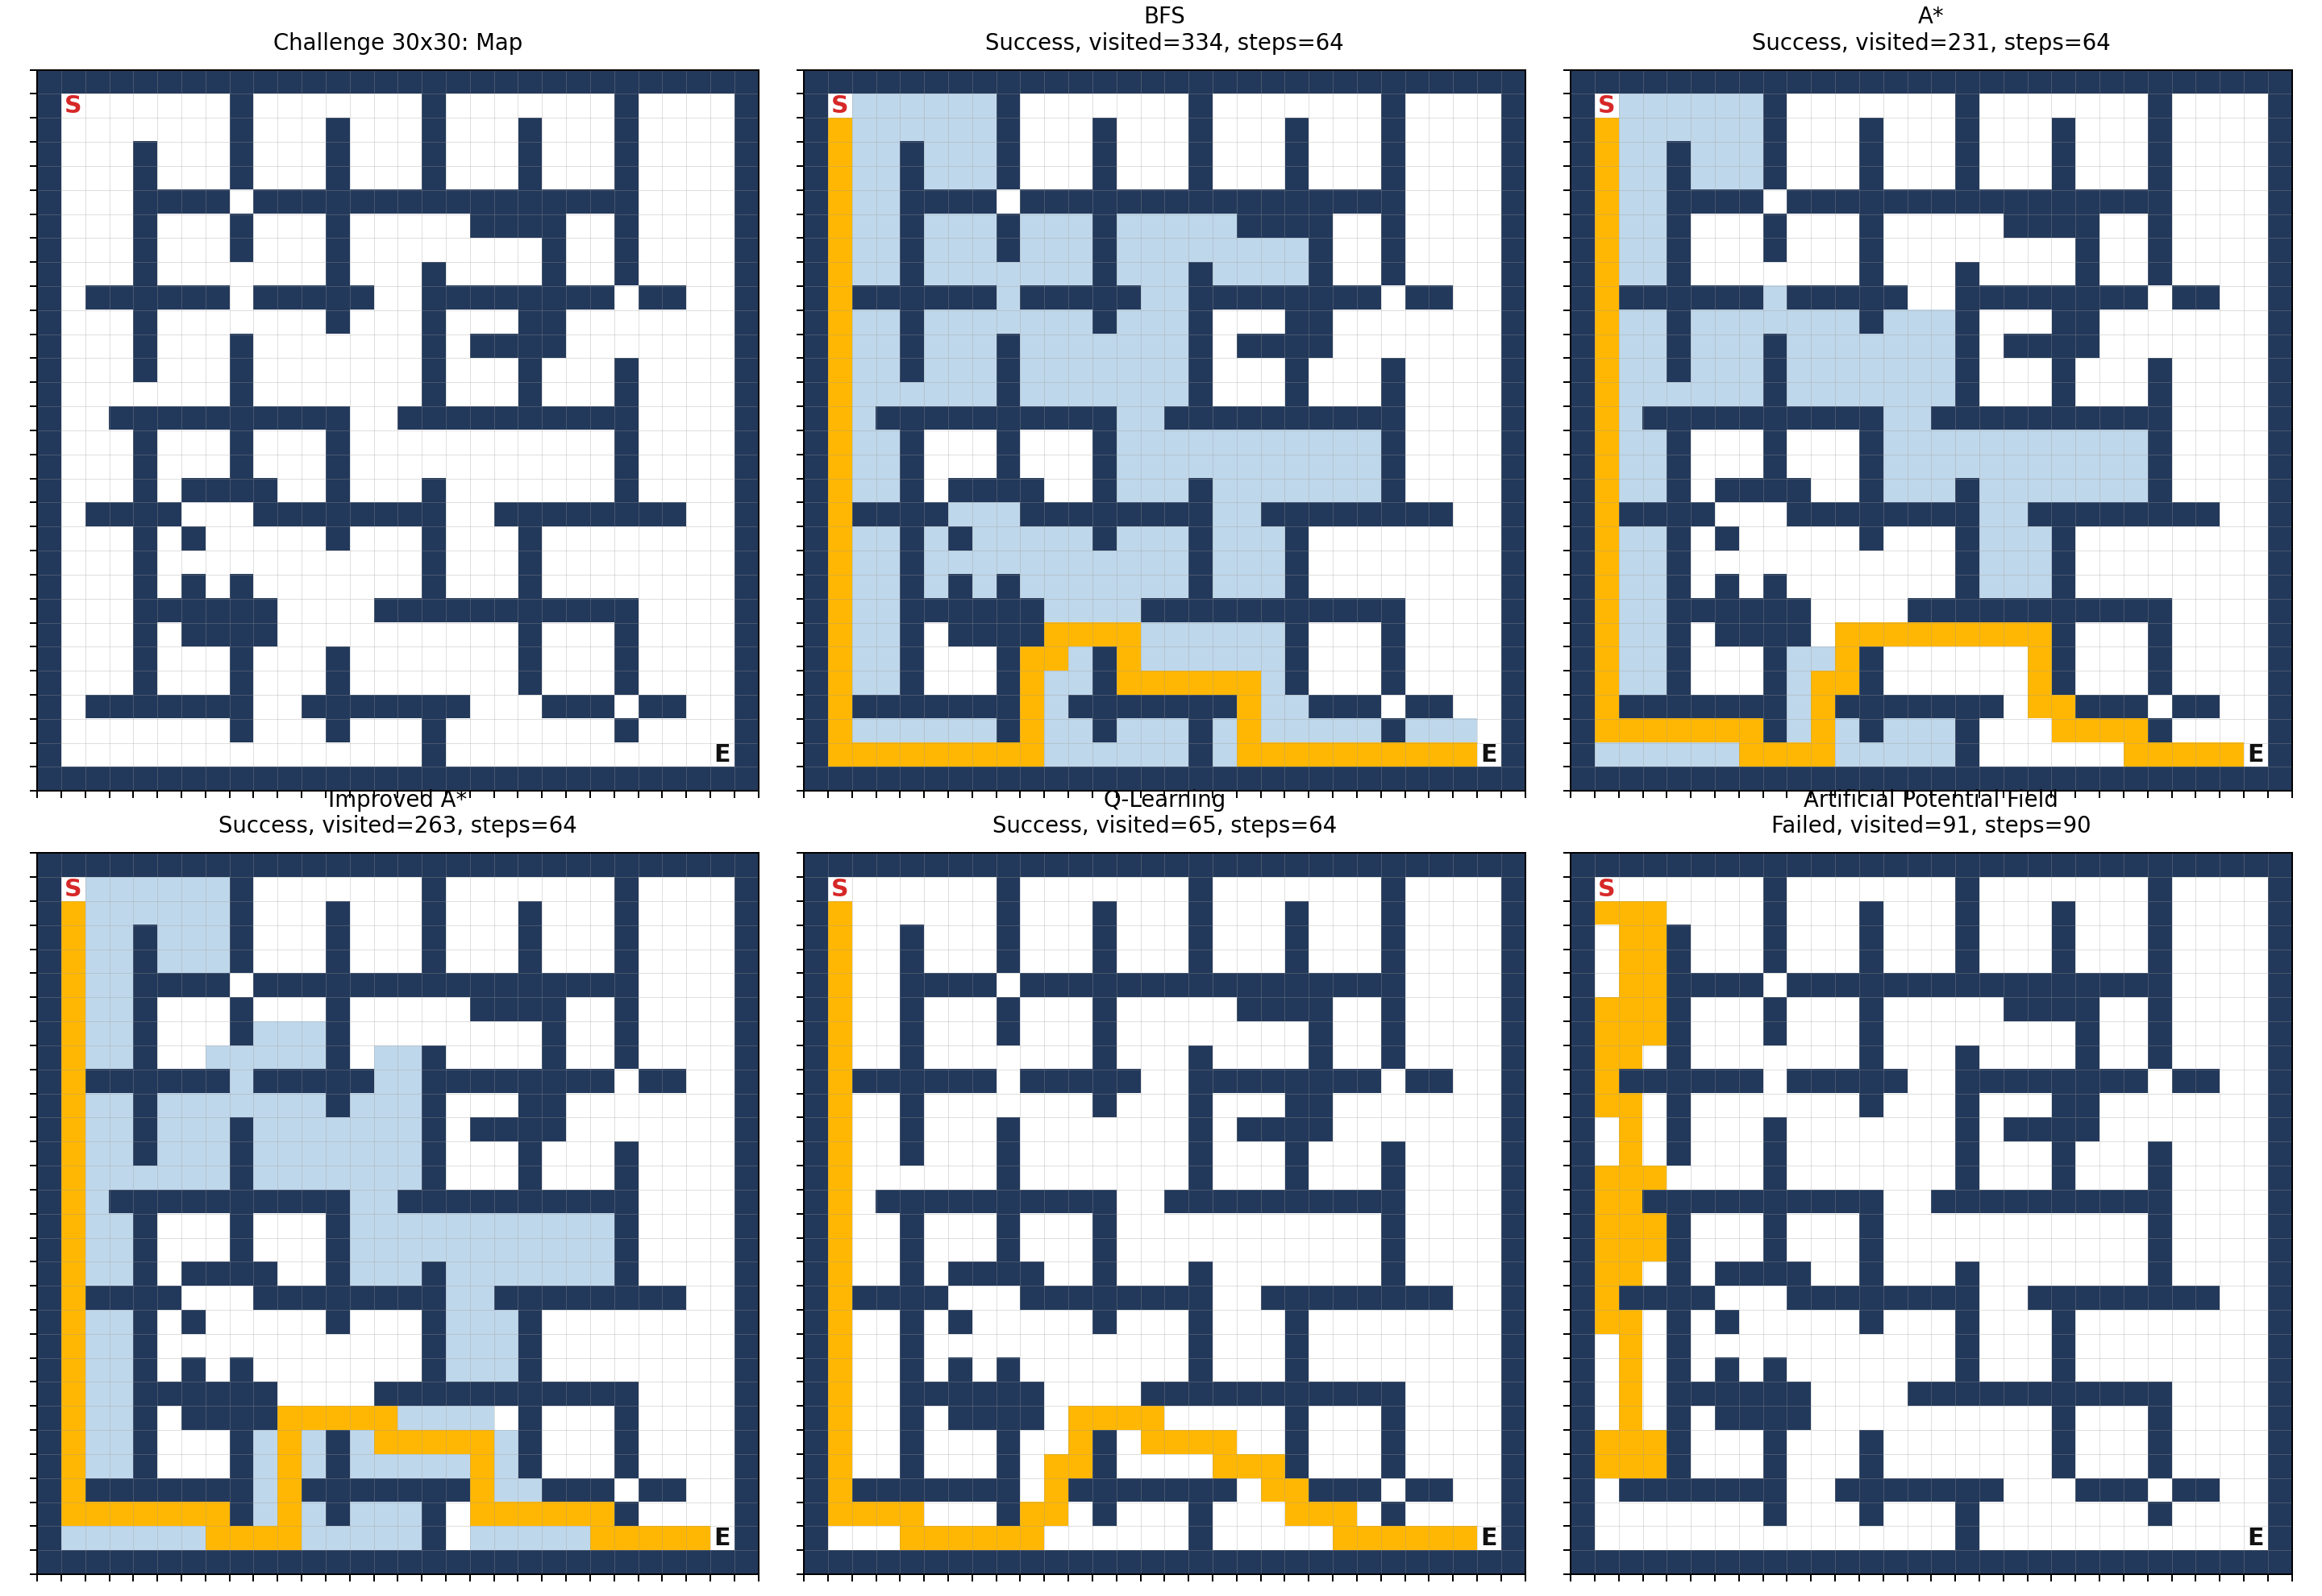
\includegraphics[width=0.93\textwidth]{../challenge_30x30_comparison.png}
  \caption{30x30 复杂场景下各算法结果对比}
  \label{fig:challenge-comparison}
\end{figure}

\begin{figure}[!htb]
  \centering
  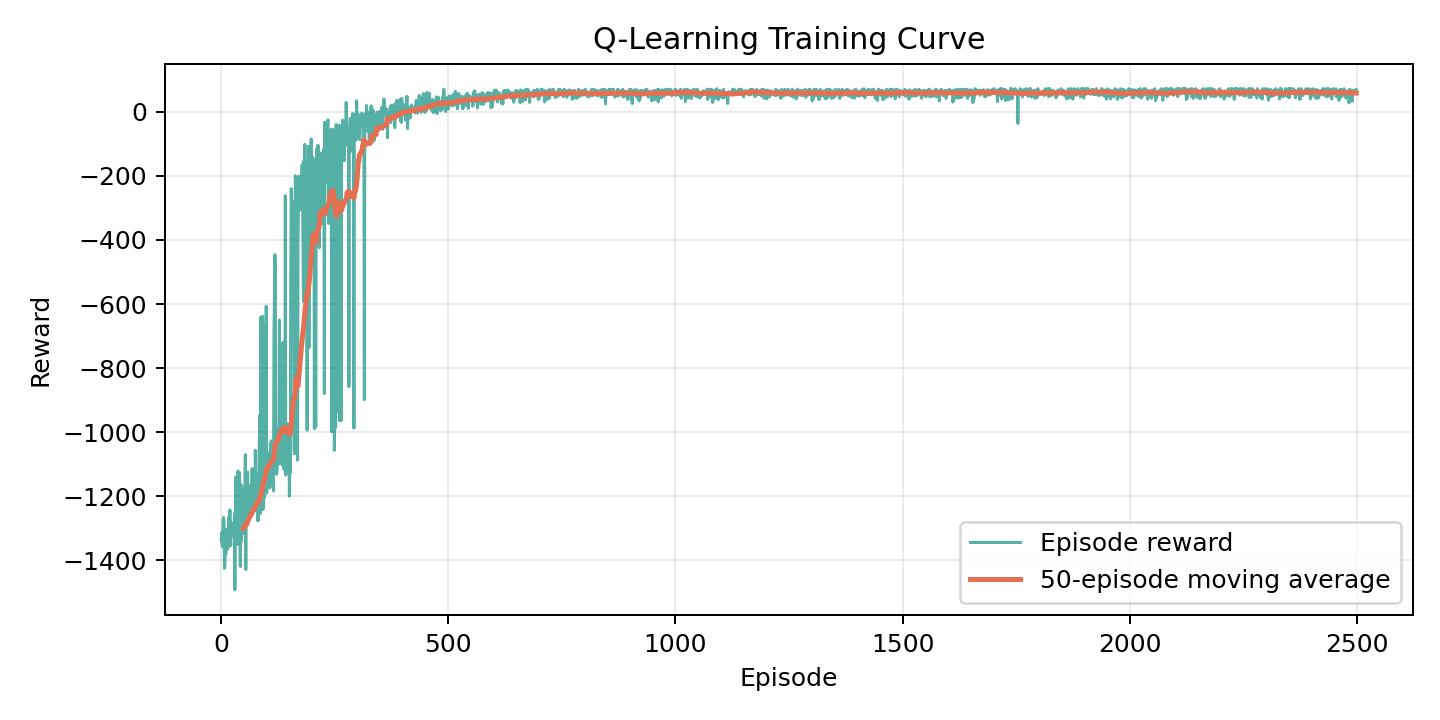
\includegraphics[width=0.72\textwidth]{../challenge_30x30_q_learning_curve.png}
  \caption{Q-Learning 在复杂场景中的训练回报曲线}
  \label{fig:qlearning-curve}
\end{figure}

\begin{figure}[!htb]
  \centering
  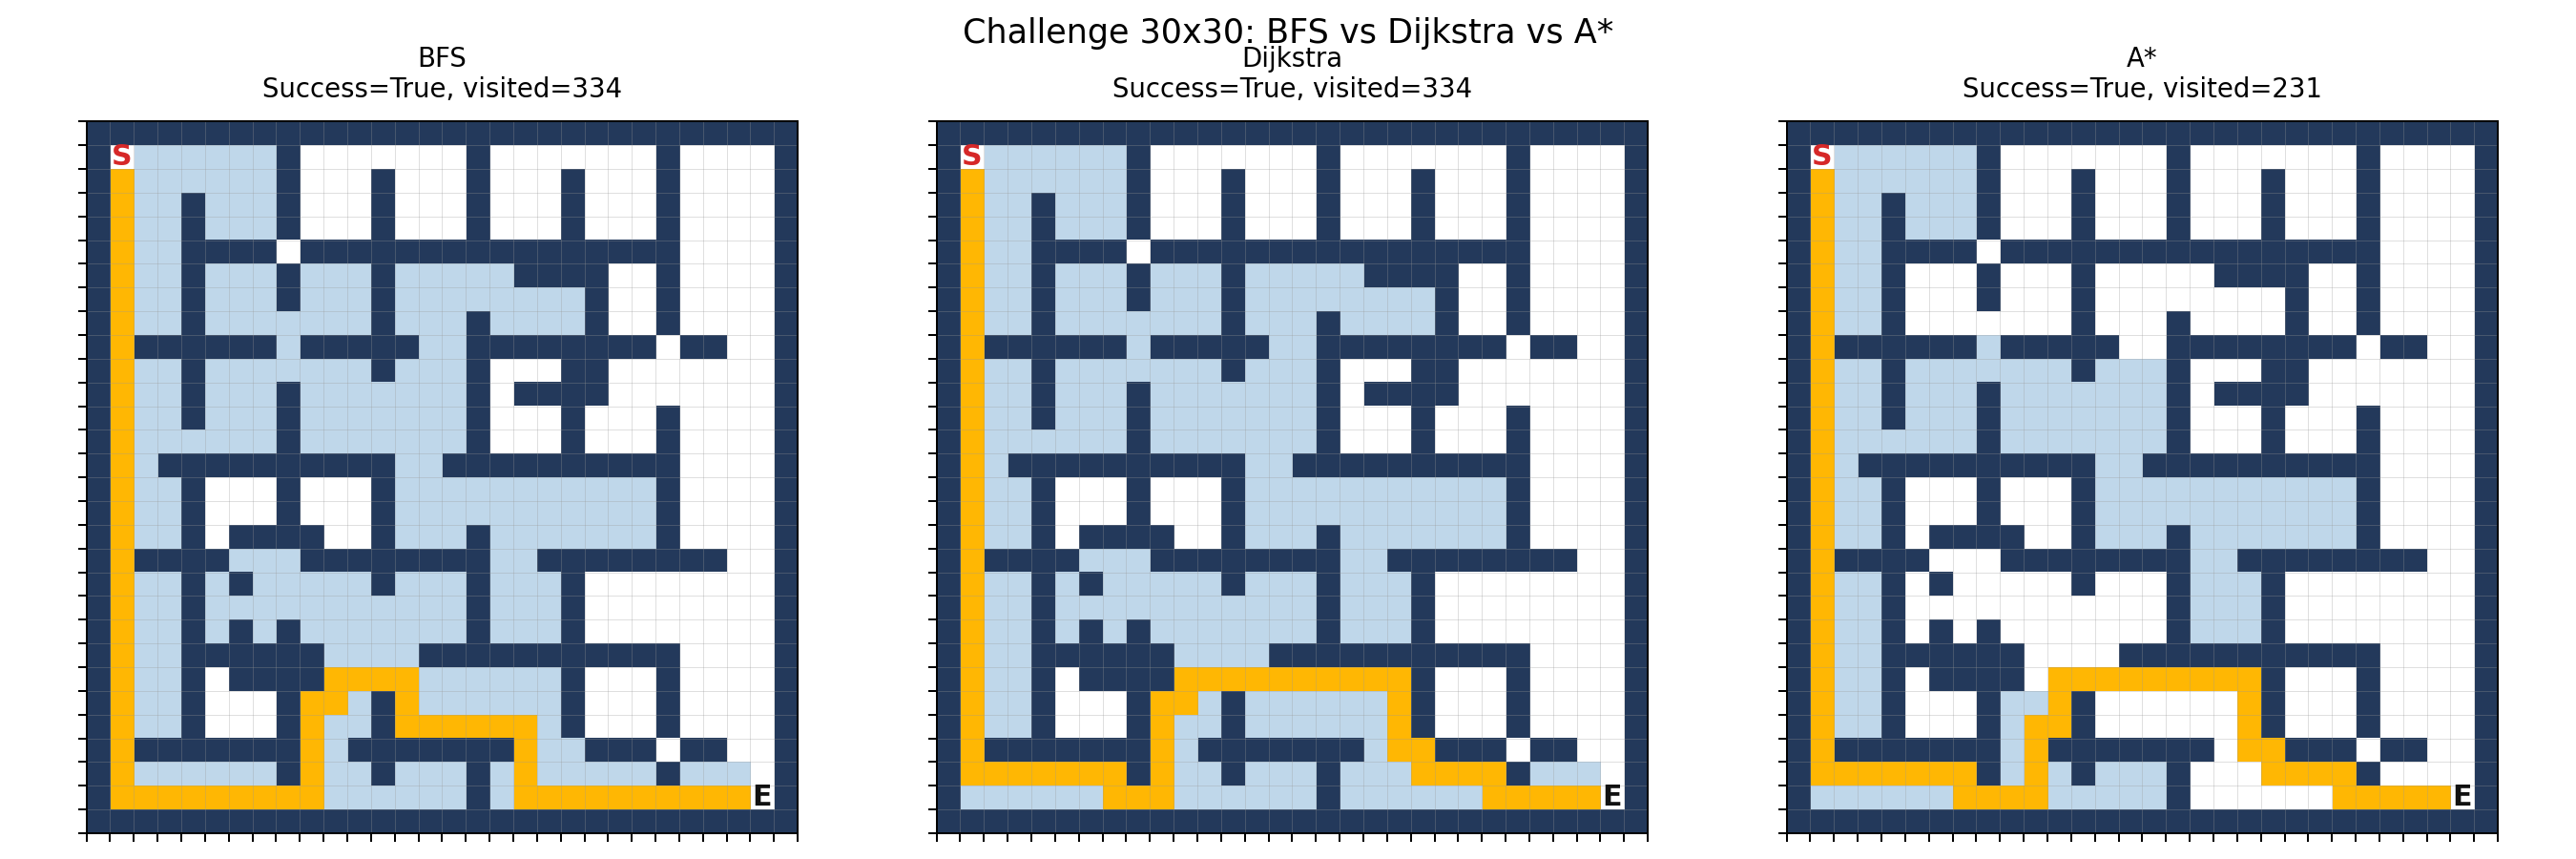
\includegraphics[width=0.78\textwidth]{../dijkstra_challenge_comparison.png}
  \caption{BFS、Dijkstra 与 A* 在复杂场景中的对比}
  \label{fig:dijkstra-comparison}
\end{figure}

\section{动态可视化结果}

为了满足题目对动态展示的要求，本文把 BFS、A* 和改进 A* 的搜索过程导出为 GIF 动画。整个动态展示分为两个阶段：

\begin{enumerate}
  \item 搜索阶段：按照节点访问顺序逐步显示已探索区域；
  \item 回溯阶段：在找到终点后逐步高亮最终路径。
\end{enumerate}

由于 PDF 不适合直接嵌入 GIF，这些动画作为随附文件提交。通过观察这些动态图，可以明显看出 BFS 的扩展更像“波纹式”铺开，而 A* 的搜索方向更集中，改进 A* 则更倾向于远离障碍区域。

\chapter{结果分析与讨论}\label{chap:analysis}

\section{不同算法的表现差异}

从实验结果可以看出，BFS 与 Dijkstra 都能够稳定找到最短路径，但在复杂场景中访问节点数很多，说明这两类算法虽然可靠，但搜索效率偏低。A* 在引入启发式函数后，访问节点明显减少，说明启发式信息确实能够有效缩小搜索范围。

改进 A* 的路径长度与普通 A* 一致，但综合代价更低，这说明加入贴障惩罚和转向惩罚后，路径质量得到了提升。虽然它的访问节点数不一定最少，但在“更安全、更平滑”这一目标上表现更好。

\section{Dijkstra 与其他算法比较}

在本文的实验中，Dijkstra 是一个很有代表性的对照算法。由于当前栅格地图中每一步的基础移动代价相同，所以 Dijkstra 与 BFS 在“是否能找到最短路径”这一点上表现接近，二者都能够稳定得到最短长度路径。但从搜索过程来看，Dijkstra 仍然需要像 BFS 一样扩展大量节点，因此在复杂场景中的效率不高。

与 A* 相比，Dijkstra 最大的区别在于它不使用终点方向信息。A* 会借助启发式函数优先扩展更接近终点的节点，所以在 30x30 场景中访问节点数明显少于 Dijkstra。这说明在静态已知地图中，启发式信息确实能够有效降低搜索范围。

与改进 A* 相比，Dijkstra 的优点是思路简单、最短路性质明确，不需要额外调参；缺点是无法表达“贴障风险”和“转弯代价”这类路径质量信息。改进 A* 虽然不一定在节点数上绝对占优，但生成的路径通常更平滑，也更符合机器人实际运动需求。

与 Q-Learning 相比，Dijkstra 不需要训练过程，结果更稳定；但它缺少学习能力，不能像强化学习方法那样通过与环境交互逐步形成策略。与人工势场法相比，Dijkstra 不会因为局部极小值问题而失败，因此在求解稳定性上更有优势。

总体来看，Dijkstra 适合作为一个“可靠但效率一般”的基准算法。在本次课程设计中，它的意义主要是提供一个无启发式最短路参考，从而更清楚地看出 A*、改进 A* 和 Q-Learning 等方法各自带来的改进效果。

\section{强化学习与启发式方法的讨论}

Q-Learning 在训练足够轮次后能够成功找到路径，说明强化学习方法在此类问题上具有可行性。相比图搜索算法，它的优势在于可以通过交互学习策略；不足之处在于训练时间较长，而且结果对奖励函数设计比较敏感。

人工势场法在简单环境中表现较直观，但在本文设计的复杂 30x30 场景中出现了失败，原因主要是 U 型障碍和窄通道导致局部极小值问题。这也说明人工势场法更适合作为局部避障方法，而不太适合单独承担复杂场景下的全局规划任务。

\section{当前方案的局限性}

虽然本文已经完成了多种算法的实现与比较，但仍存在一些局限：

\begin{itemize}
  \item 当前地图是静态已知环境，没有加入动态障碍；
  \item 机器人运动方式只考虑上下左右四个方向，没有考虑速度和转向半径等真实约束；
  \item Q-Learning 仍然是表格型实现，状态规模扩大后训练成本会快速增加；
  \item 动态展示目前以 GIF 形式导出，交互性还不够强。
\end{itemize}

\section{可改进方向}

后续可以从以下几个方向继续改进：

\begin{enumerate}
  \item 引入 D* Lite、LPA* 等增量式搜索算法，处理动态环境变化；
  \item 将 Q-Learning 扩展为深度强化学习方法，提升大规模场景下的泛化能力；
  \item 在代价函数中进一步加入转弯半径、安全距离等约束，使路径更贴近真实机器人需求；
  \item 设计更丰富的可视化界面，实现交互式播放和参数调节。
\end{enumerate}

\chapter{总结}\label{chap:summary}

本次课程设计围绕机器人避障寻径问题，完成了从基础算法实现、复杂场景设计，到多算法比较和动态可视化展示的一整套实验流程。

具体来说，本文首先实现了 BFS 和 A* 两种基础算法；随后自主设计了一个 30x30 的复杂障碍场景；在此基础上补充实现了改进 A*、Q-Learning、人工势场法和 Dijkstra；最后输出了静态结果图、训练曲线和 GIF 动态展示文件。

实验结果表明：
\begin{itemize}
  \item BFS 和 Dijkstra 能稳定得到最短路径，但搜索范围较大；
  \item A* 具有更高的搜索效率；
  \item 改进 A* 能在路径长度不变的前提下降低综合代价；
  \item Q-Learning 经过训练后能够得到可行路径；
  \item 人工势场法在复杂环境中容易受到局部极小值影响。
\end{itemize}

总体来看，本次课程设计让我对图搜索算法、强化学习方法以及路径规划中的可视化展示有了更直观的理解。


\end{document}
